\chapter{界面设计}
在本章节中将展示web前端界面,来源于demo设计,采用扁平化设计风格,pc和手机端均可通过网页登录系统,此处选用手机端的界面,pc端界面类似。
\section{注册界面}
\begin{figure}[H]
	\centering
	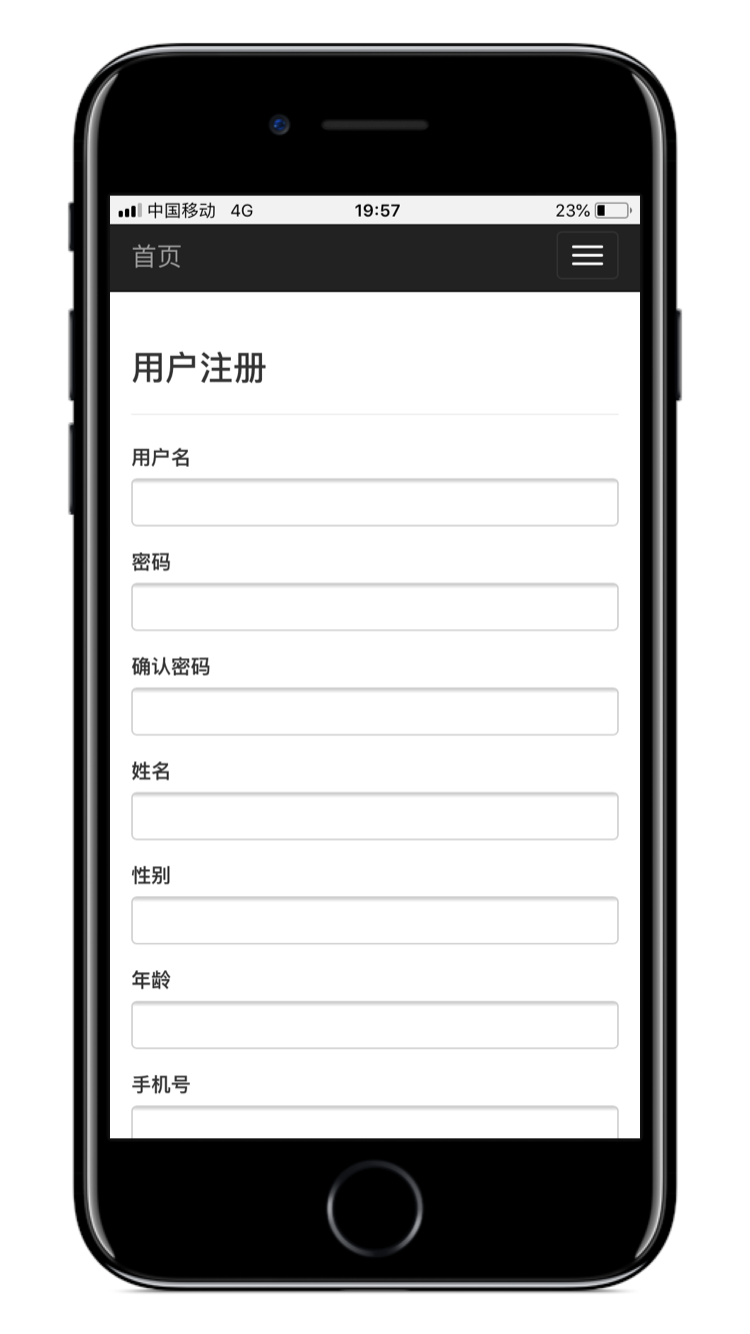
\includegraphics[width=9cm]{register.PNG}
	\caption{注册界面} 
	\label{fig:figure1}
\end{figure}


\section{登录界面}
\begin{figure}[H]
	\centering
	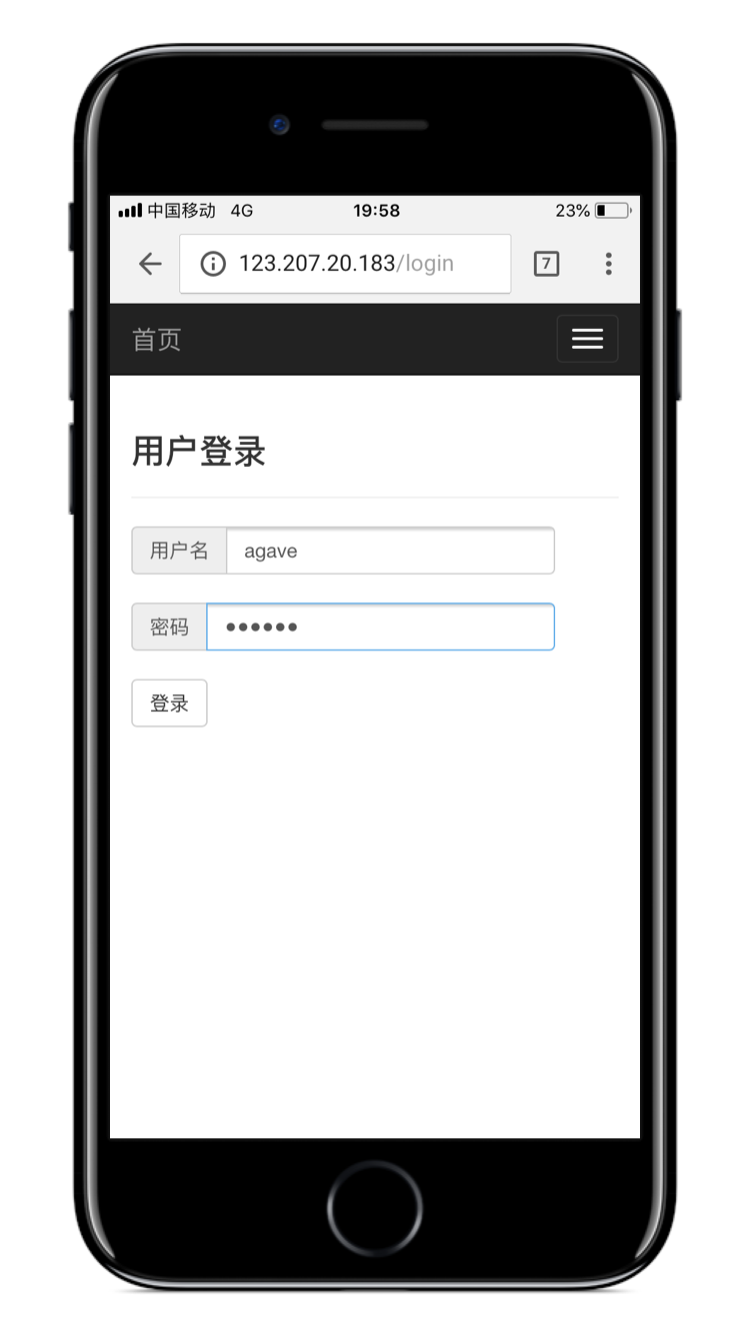
\includegraphics[width=9cm]{login.PNG}
	\caption{登录界面} 
	\label{fig:figure2}
\end{figure}
在登录界面,用户输入用户名和密码然后点击登录后提交到服务器后台进行验证。

\section{菜单界面}
\begin{figure}[H]
	\centering
	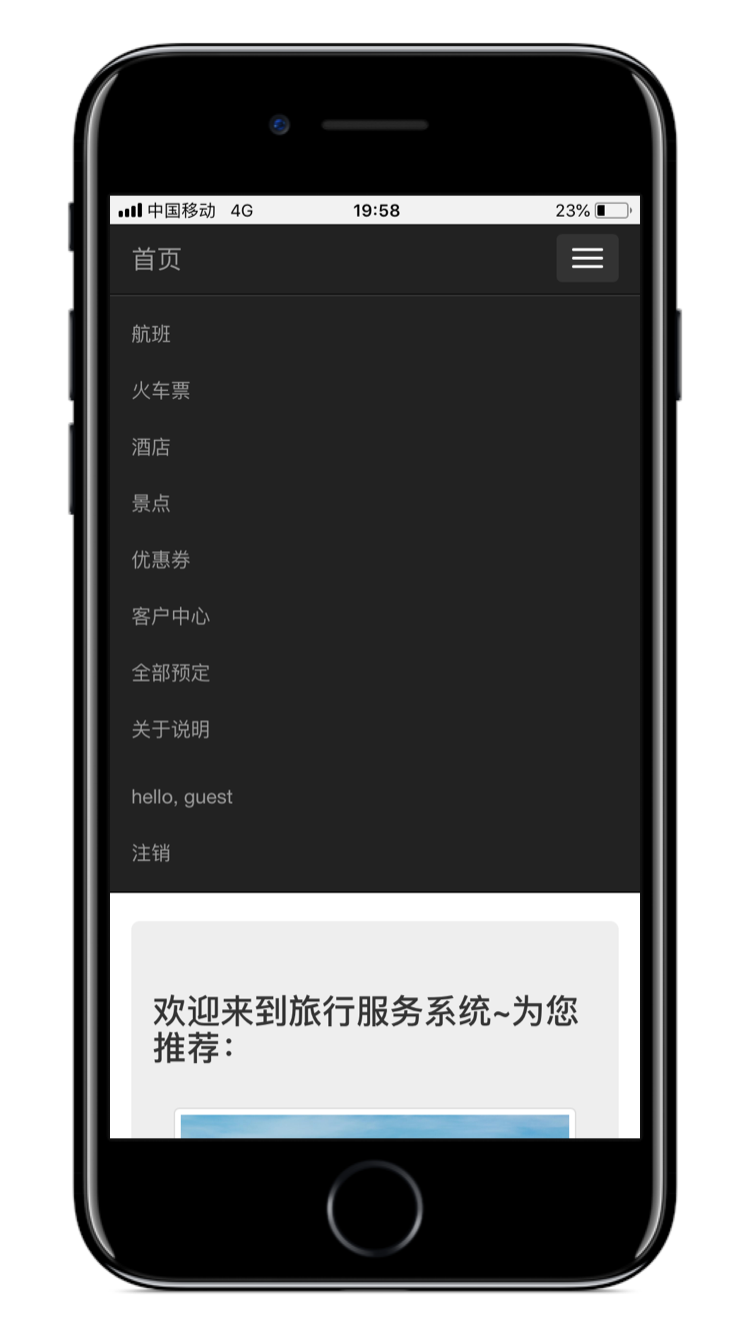
\includegraphics[width=9cm]{menu.PNG}
	\caption{菜单界面} 
	\label{fig:figure3}
\end{figure}
此处展示的为整个web前端界面的顶部菜单栏,在pc端全部显示,在手机端点击右边的展开选项后即可看到所有的菜单选项进行选择。


\section{主页界面}
\begin{figure}[H]
	\centering
	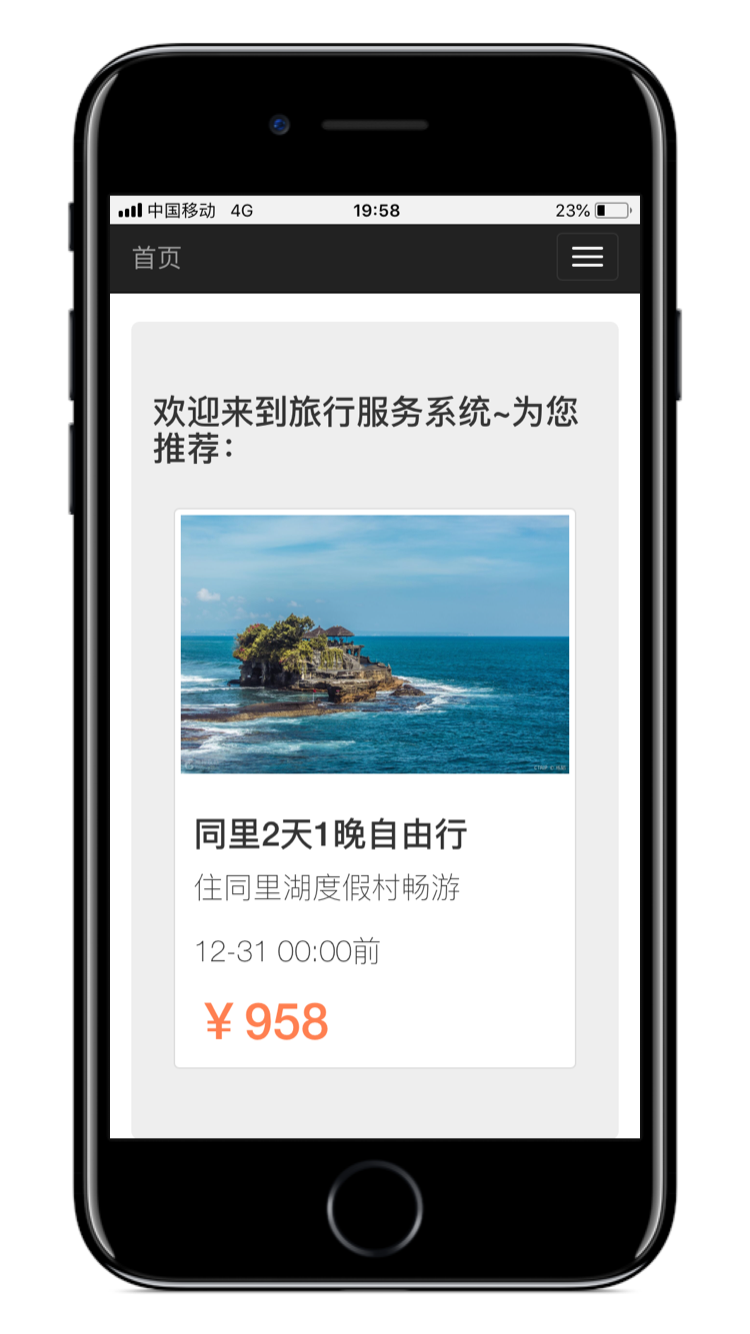
\includegraphics[width=9cm]{index.PNG}
	\caption{主页界面} 
	\label{fig:figure4}
\end{figure}
主页界面向用户推送广告活动。


\section{航班预订界面}
\begin{figure}[H]
	\centering
	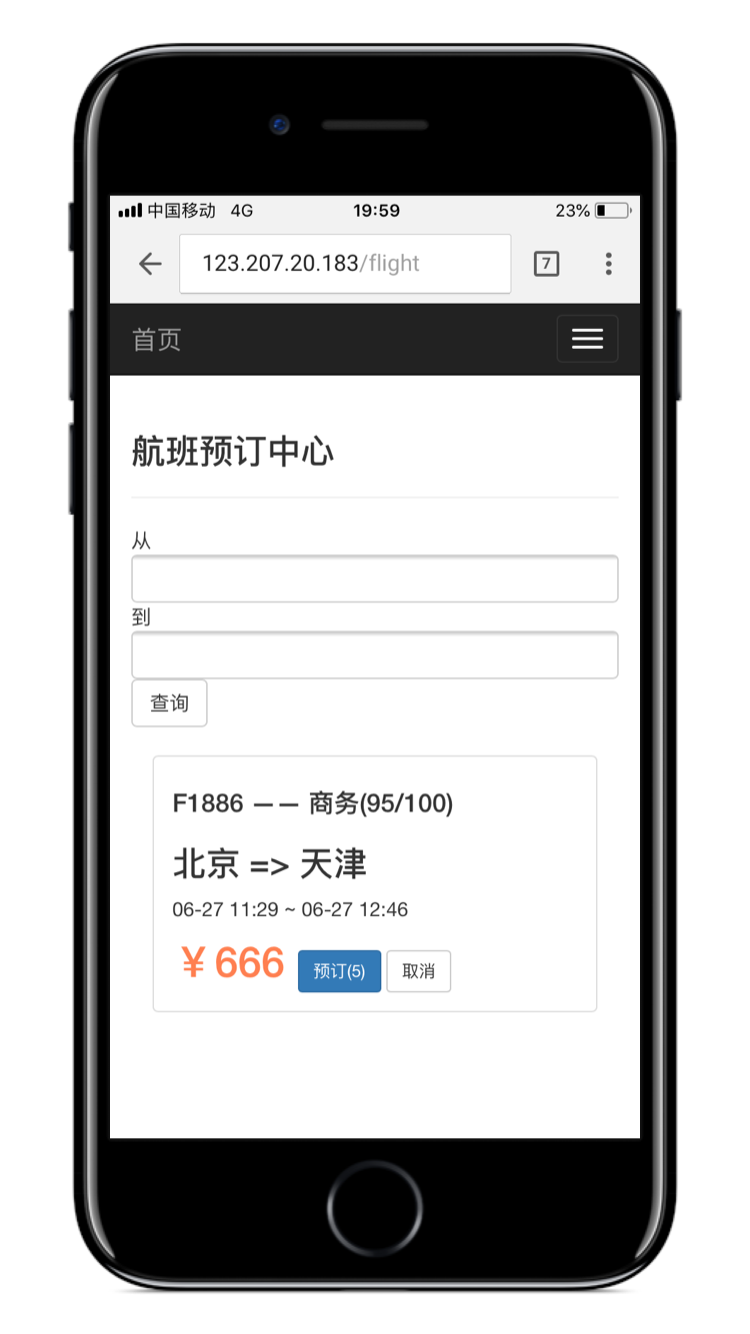
\includegraphics[width=9cm]{flight.PNG}
	\caption{航班预订界面界面} 
	\label{fig:figure5}
\end{figure}
在航班预订界面,用户可以浏览到所有的航班信息,同时有一个预订按钮,用户点击后即可预订数+1,并且即时显示预订数量,同时也可以取消预订。


\section{火车票预订界面}
\begin{figure}[H]
	\centering
	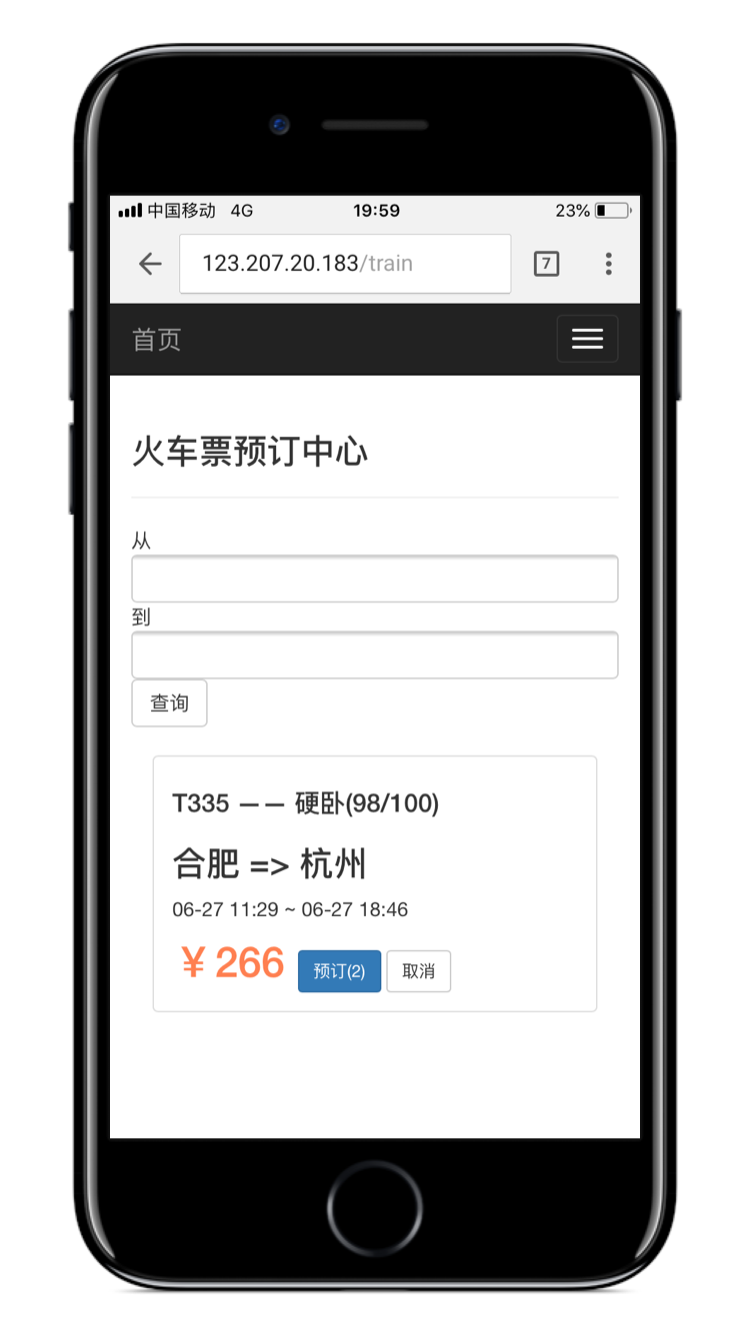
\includegraphics[width=9cm]{train.PNG}
	\caption{火车票预订界面} 
	\label{fig:figure6}
\end{figure}
在火车票预订界面,用户可以浏览到所有的火车票信息,同时有一个预订按钮,用户点击后即可预订数+1,并且即时显示预订数量,同时也可以取消预订。


\section{酒店预订界面}
\begin{figure}[H]
	\centering
	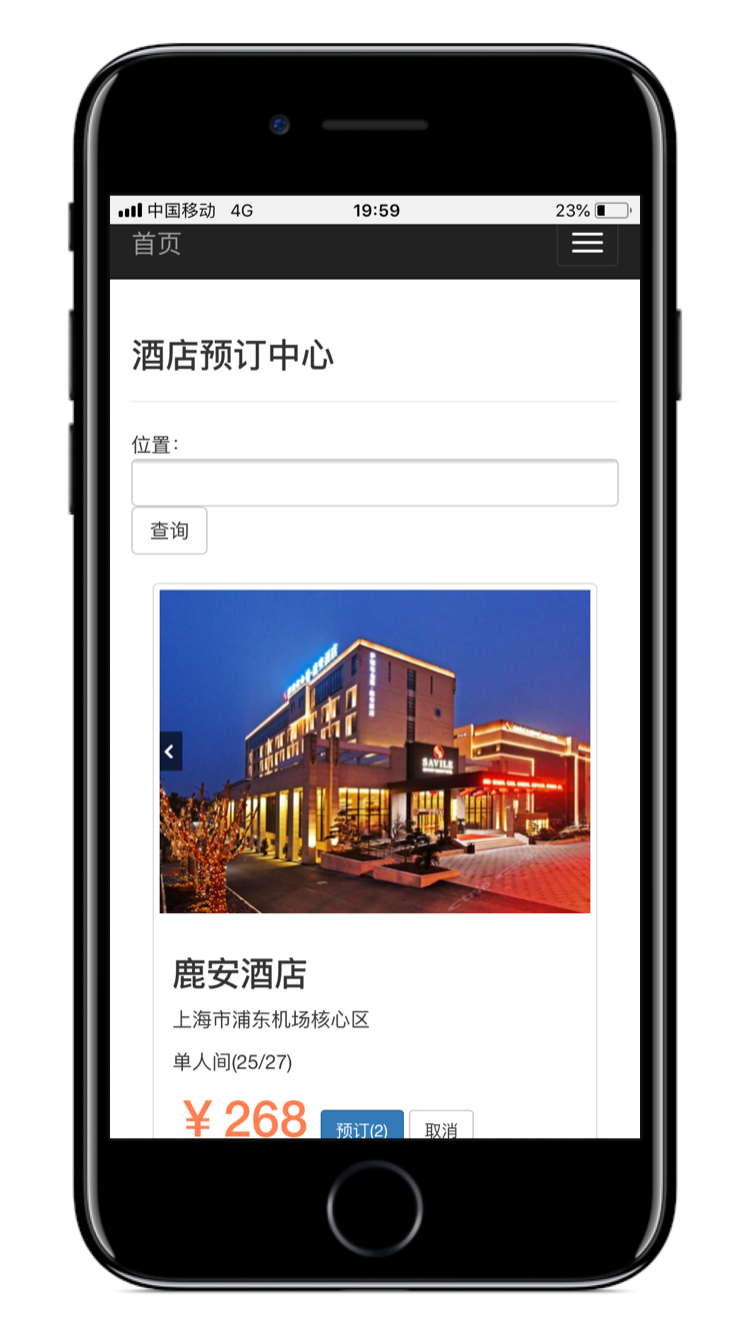
\includegraphics[width=9cm]{hotel.PNG}
	\caption{酒店预订界面} 
	\label{fig:figure7}
\end{figure}
在酒店预订界面,用户可以浏览到所有的酒店信息,同时有一个预订按钮,用户点击后即可预订数+1,并且即时显示预订数量,同时也可以取消预订。


\section{景点预订界面}
\begin{figure}[H]
	\centering
	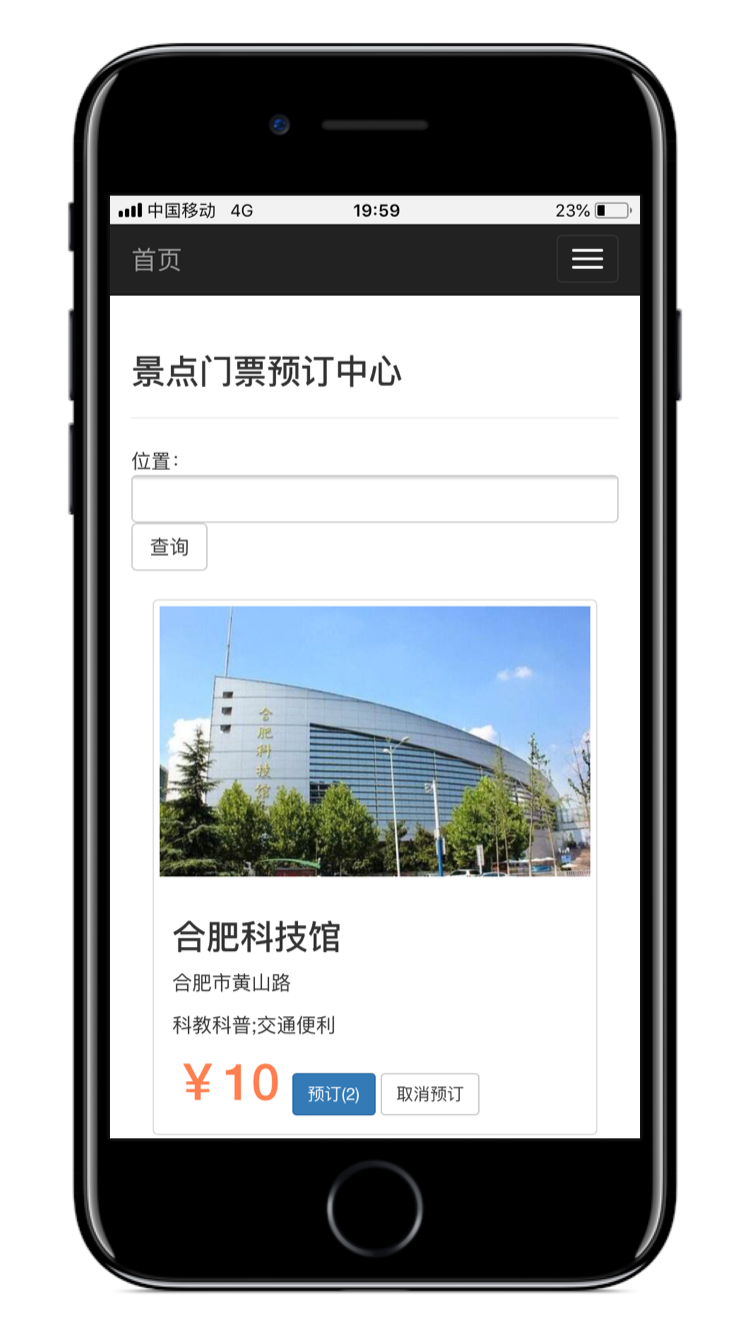
\includegraphics[width=9cm]{attraction.PNG}
	\caption{景点预订界面} 
	\label{fig:figure8}
\end{figure}
在景点门票预订界面,用户可以浏览到所有的景点信息,同时有一个预订按钮,用户点击后即可预订数+1,并且即时显示预订数量,同时也可以取消预订。



\section{优惠券领取界面}
\begin{figure}[H]
	\centering
	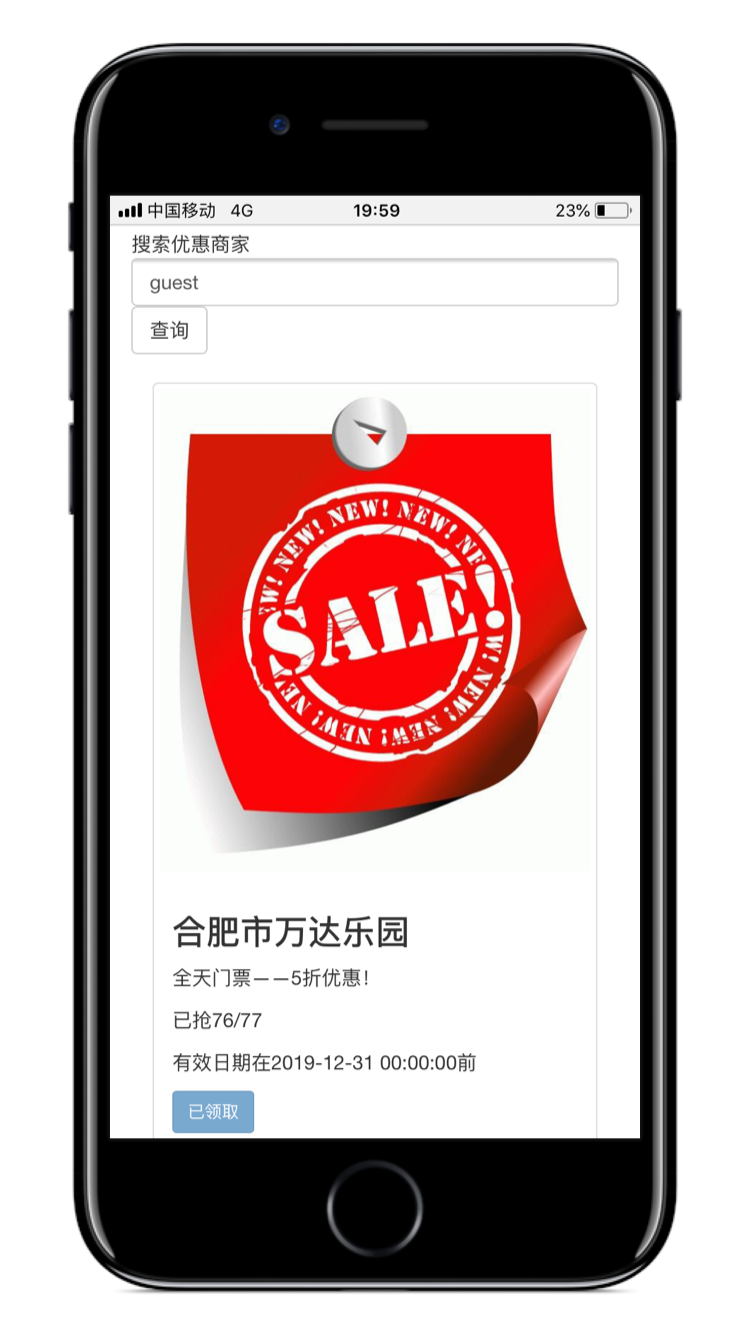
\includegraphics[width=9cm]{coupon.PNG}
	\caption{优惠券领取界面} 
	\label{fig:figure9}
\end{figure}
在优惠券领取界面,用户可以浏览到所有的优惠券信息,同时有一个领取按钮,用户点击后即可领取该优惠券,并且即时显示"已领取",无法重复领取。



\section{个人信息界面}
\begin{figure}[H]
	\centering
	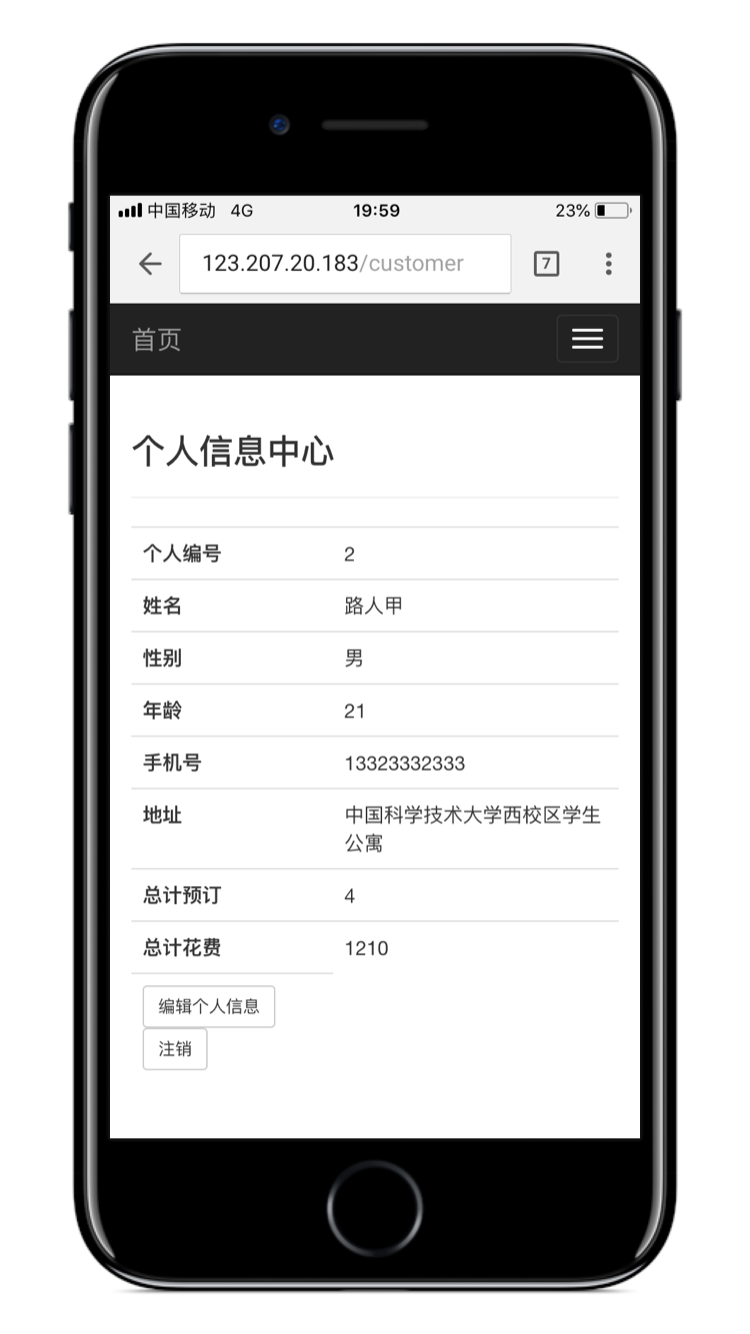
\includegraphics[width=9cm]{customer.PNG}
	\caption{个人信息界面} 
	\label{fig:figure10}
\end{figure}
在此界面用户可以看到个人所有的信息,并且可以进行注销或者编辑个人信息。


\section{预订信息界面}
\begin{figure}[H]
	\centering
	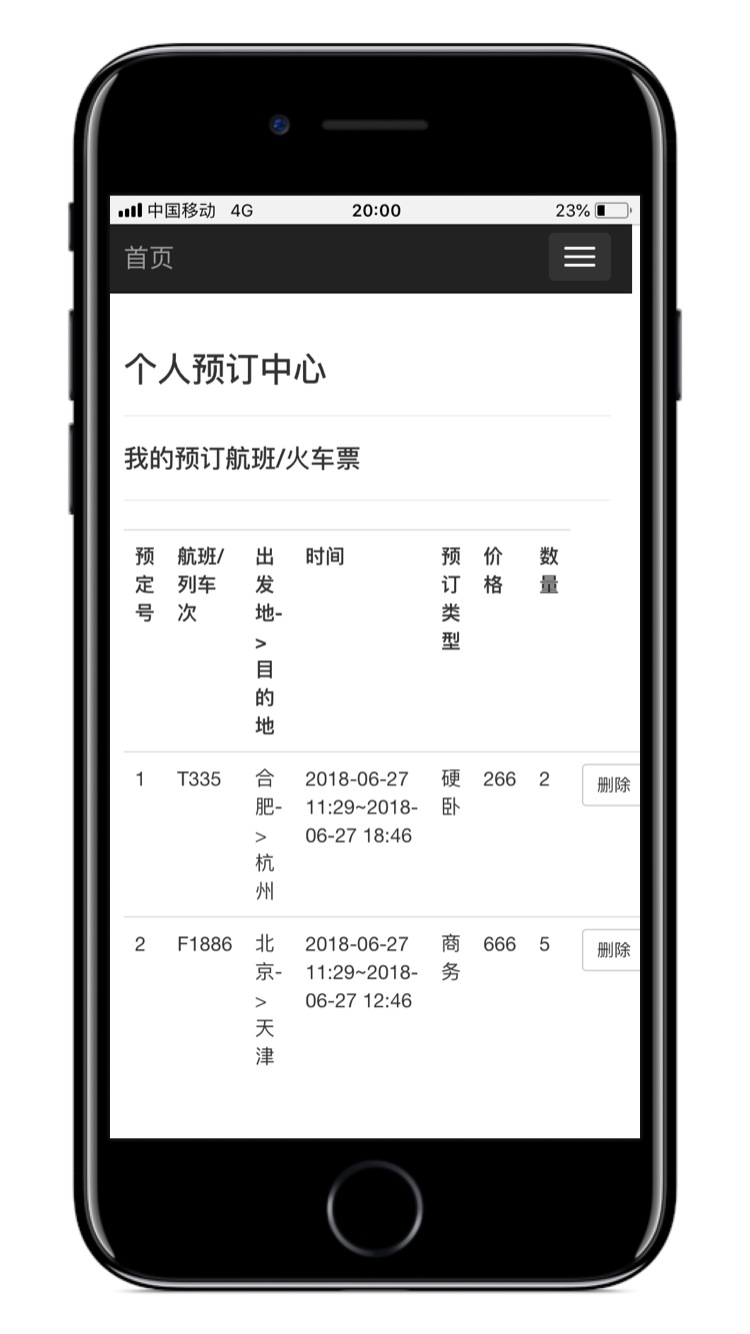
\includegraphics[width=9cm]{reservation.PNG}
	\caption{火车票预订界面} 
	\label{fig:figure11}
\end{figure}
在预订信息界面,用户可以看到自己的全部预订信息,包括每一项的预订数量以及时间等详细说明。

\section{编辑信息界面}
\begin{figure}[H]
	\centering
	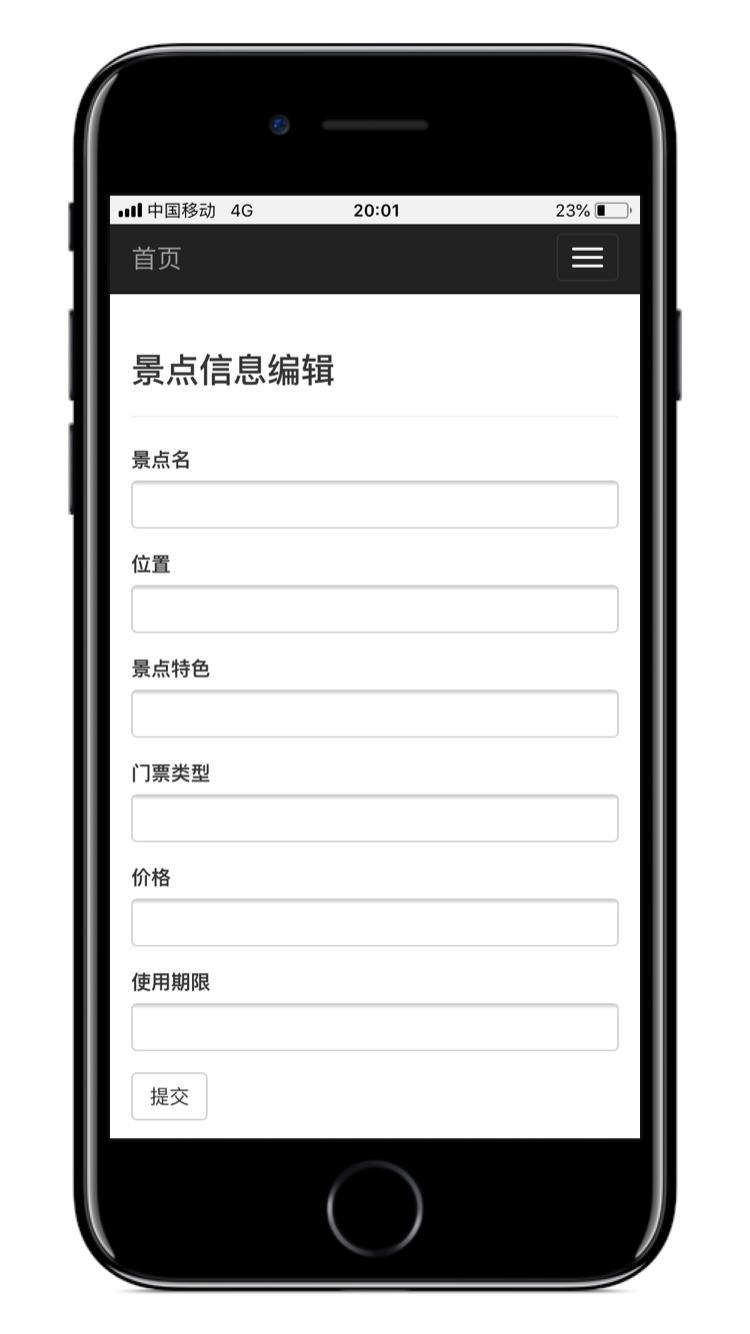
\includegraphics[width=9cm]{edit.PNG}
	\caption{编辑信息界面} 
	\label{fig:figure12}
\end{figure}
当管理员登录时,会提供每一个模块类别的编辑信息,管理员可以增加新的项目或者进行编辑,此处仅仅展示其中一个编辑界面,航班/火车票等模块的编辑界面类似。
